F\"ur die digitale  Logik  werden  die  zwei  Spannungspegel  \SI{5}{\volt}  und
\SI{3.3}{\volt} ben\"otigt.

\begin{figure}[th!]
    \center
    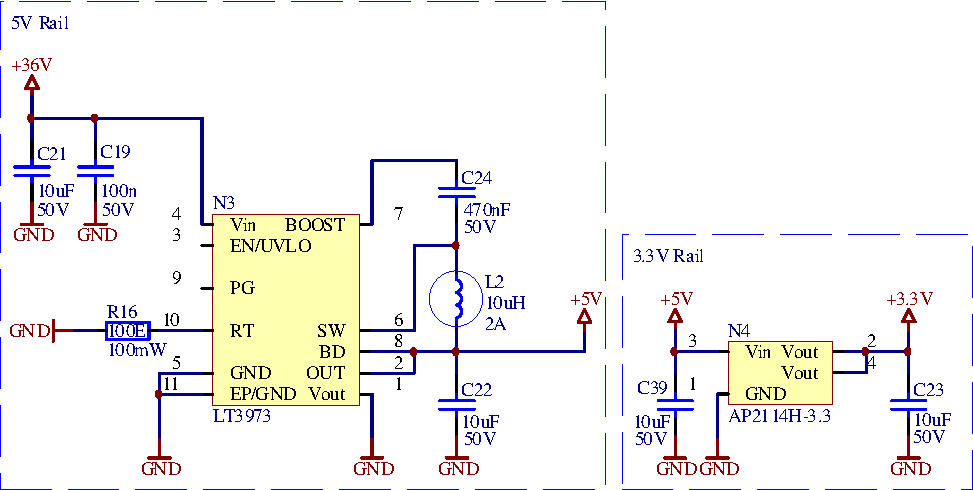
\includegraphics[width=.75\textwidth]{images/circuit/5v-3v-rails.pdf}
    \caption{Speisung f\"ur 5V mittels Abwertswandler (links) und Speisung f\"ur 3.3V mittels Linearregler (rechts)}
    \label{fig:circuit:rails}
\end{figure}

Die  \SI{36}{\volt} vom Netzteil werden mittels eines getakteten  DC-DC-Wandlers
auf \SI{5}{\volt} transformiert,  was  in  der Abbildung \ref{fig:circuit:rails}
vom Bauteil $N_3$ verwirklicht wird.

Die  \SI{5}{\volt}  werden  von  einem  Linearregler  $N_4$ auf  \SI{3.3}{\volt}
gestuft. Ein Linearregler wurde  gew\"ahlt  damit  die  \SI{3.3}{\volt} Speisung
m\"oglichst  St\"orfrei  bleibt  --  Getaktete  Wandler  verursachen  viel  mehr
St\"orung. Somit  wird  verhindert,  dass  die DACs und ADCs verrauscht sind und
ungenau messen.
